\section{Teleoperated Manipulation Method}
	\label{sec:teleop_manip_method}
	
	Let us consider a humanoid robot equipped with a Laser Range Finder (LRF) placed at the head,
	as well as three cameras: at the head and at each hand.
	The LRF provides a point cloud of the environment, probably contaminated with noise due to the enviromental
	conditions of the disaster scenario; that is, even after a proper calibration it is not possible to consider
	that the 3D data precisely represents points belonging to objects in the environment, but within a certain
	amount of tolerance.
	On the other hand, the frame rate of the cameras, as well as the resolution, are intentionally set low
	foreseeing the effects of the degraded communication.
	
	This information of the environment, together with the sensorial information providing the current state of
	the robot, are the only information available to the operator, which has to supervise the robot while performing
	the tasks by establishing	high level goals, assisting with perception and changing parameters during the task.
	For this purpose, and under the circumstances stated above, we came up with a teleoperated manipulation method
	based on ``markers'' which assume minimum knowledge of the environment.
	This one is explained on the following.
	
	\subsection{Approaching to the target}
	
		The robot must achieve a proper stance with respect to the object(s) representing the target of the task,
		such that they be inside of the dextrous workspace of the hands of the robot.
		To do that the robot must perform a first measurement of the environment in order to check, together with the
		head camera, if the manipulation target is represented by some set of points of the resulting point cloud.
		In such a case, a preliminar alignment of a 3D object representing this manipulation target
		(the \emph{manipulation marker}) is first performed.
		
		By using the Graphical User Interface (GUI) provided by Choreonoid\cite{Nakaoka_Choreonoid}, the Manipulation
		Marker is represented as the corresponding 3D model together with a set of arrows and rings which allow the
		operator to translate and rotate it with respect to its local reference frame,
		as depicted in \figurename~\ref{fig:ManipulationMarker}.
		
		\begin{figure}[b]
			\centering
			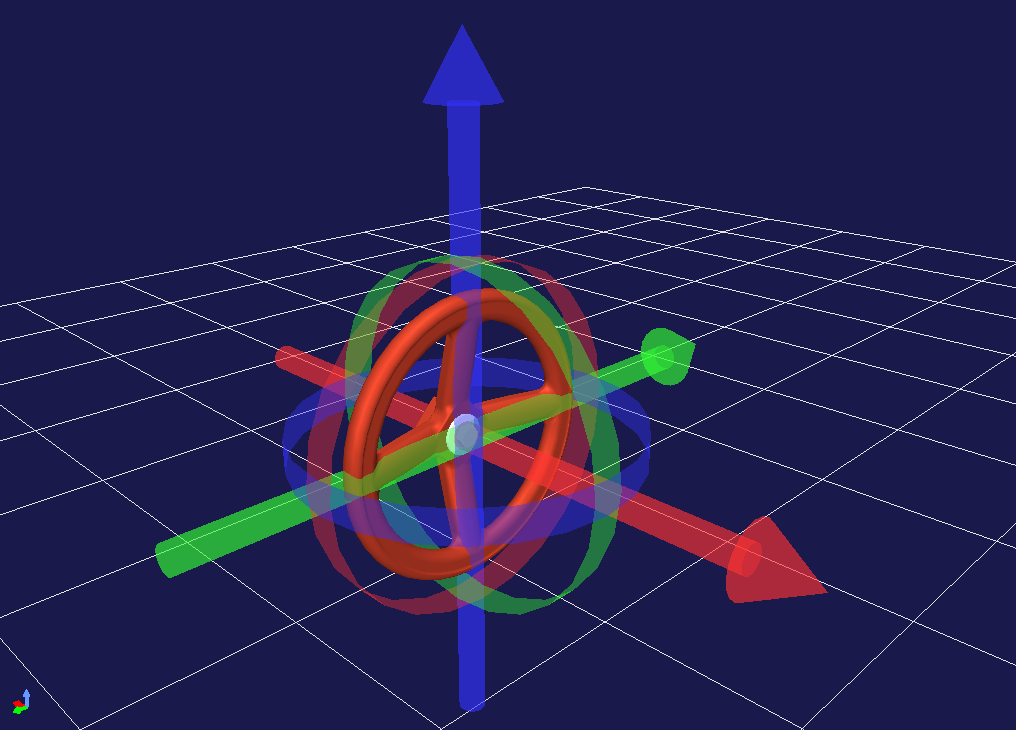
\includegraphics[height = 5.5cm]{img/ManipulationMarker}
			\caption{Manipulation Marker of a valve.}
			\label{fig:ManipulationMarker}
		\end{figure}

		Doing this alignment manually can be tedious, besides the fact that it may require a lot of time.
		To speed it up, it is possible to use a built in function included in the Point Cloud Library (PCL) that
		automatically alignes the marker with the best fit set of points, by providing maximum displacements,
		the number of iterations and some allowable error.
		However, ordinarily the robot will not be close enough to the object(s) for them to be measured with enough
		density of points, in such a way that the automatic alignment be prone to fail.
		One way to overcome this problem is to select one point of the point cloud belonging to the object and set
		this as the origin of the local reference frame of the Manipulation Marker, then the automatic alignment
		will lead to an alignment that may or may not require further small manual adjustments.
		
		One way to improve the initial alignment of the Manipulation Marker is to use beforehand information of the
		possible attitude of the object with respect to the nearest wall.
		For example, if the manipulation target is a box attached to the wall, its front face will probably be
		parallel to it.
		Knowing this, it is just the matter to identify the plane of the wall (and maybe the floor),
		get its mathematical representation and use it to define an initial attitude of the Manipulation Marker,
		requiring little automatic or manual adjustments.
		
		Once this is done, it is possible to define a proper stance of the robot (calculated beforehand) with respect
		to the local reference frame of the Manipulation Marker.
		Then, by taking into account the height field of the floor (obtained from the point cloud) and avoiding the
		obstacles of the environment (walls and/or other objects), a proper footstep planning is performed in order
		for the humanoid robot to arrive to the desired stance.
		
	\subsection{Grasping the target}
		
		Once humanoid the robot arrives to the desired stance, it has to perform another measurement.
		First, because of the positioning errors accumulated during its locomotion, and second,
		in order to obtain a more dense point cloud inteded for refining the alignment of the Manipulation Marker.